%---------------
%╔═╗╔═╗╔╦╗╦ ╦╔═╗
%╚═╗║╣  ║ ║ ║╠═╝
%╚═╝╚═╝ ╩ ╚═╝╩  
%---------------
\documentclass[12pt,oneside,a4paper]{report}

% DOCUMENT SETUP
\usepackage[left=3cm, 
			right=2.5cm, 
			top=2.5cm, 
			bottom=2.5cm, 
			includehead, 
			includefoot]{geometry}

% line spacing
\usepackage{setspace}
\setstretch{1,25} % 15/12 --> 1.25

%de­fines Adobe Times Ro­man as de­fault text font
\usepackage{mathptmx}
\usepackage{times} % needed for acronym package

%PDF linking package
\usepackage[hidelinks]{hyperref}

% Language Setup
\usepackage[ngerman]{babel}
% language specific bibliography style
\usepackage[numbers]{natbib}
\usepackage[fixlanguage]{babelbib}
\selectbiblanguage{german}
% bliographystyle setup
% default style names: apalike alphadin ieeetr IEEEtranSN apalike2 alphadin 
% babel specific: babplain, babplai3, babalpha, babunsrt, bababbrv, bababbr3 unsrt 
\bibliographystyle{unsrturl}

% encoding setup
% T1 font encoding for languages that use a latin alphabet
\usepackage[T1]{fontenc} 

% enhanced input encoding handling - utf8 for äÄüÜöÖß...
\usepackage[utf8]{inputenc}
%\usepackage{ucs}%utf8x suppart

% after babel - set chapter string
\AtBeginDocument{\renewcommand{\chaptername}{}}

% enumeration
\usepackage{enumitem}
% tabular extension tabularx
\usepackage{tabularx}

% math packages
\usepackage{amsmath}
\usepackage{nicefrac}
\usepackage{amsthm}
\usepackage{amsbsy}
\usepackage{amssymb}
\usepackage{amsfonts}
\usepackage{MnSymbol}

% patches for latex
\usepackage{fixltx2e}

%special characters
\usepackage{amssymb}
\usepackage{upgreek,textgreek}

% acronym package
\usepackage[printonlyused, footnote]{acronym}

% breakable text in \seqsplit{}
\usepackage{seqsplit}

% \textmu
\usepackage{textcomp}

% package provides a way to compile sections of a document using the same preamble as the main document
\usepackage{subfiles}

% driver-independent color extension - used by listings,tabularx
\usepackage[usenames,dvipsnames,table,xcdraw]{xcolor}

% -- SYNTAX HIGHLIGHTING --
\usepackage{listings}
%% bash command line Syntax Highlighting
\lstdefinestyle{BASH_CMD}{ 
  columns=fullflexible,            % copy pasteable listings
  language=bash,
  basicstyle=\small\sffamily,
  basicstyle   = \small \ttfamily,
  keywordstyle = [1]\small \ttfamily,
  keywordstyle = [2]\small \ttfamily,
  commentstyle = \small \ttfamily,
  numbers=none,
  captionpos=b, 
  breaklines=true,
  numberstyle=\tiny,
  numbersep=3pt,
  frame=tlrb,
  columns=fullflexible,
  backgroundcolor=\color{white!20},
  linewidth=\linewidth,
  literate=                        % replace in code
     {Ö}{{\"O}}1
     {Ä}{{\"A}}1
     {Ü}{{\"U}}1
     {ß}{{\ss}}2
     {ü}{{\"u}}1
     {ä}{{\"a}}1
     {ö}{{\"o}}1
}
 % adds style BASH_CMD
%% Matlab Syntax Highlighting
\colorlet{keyword}{blue!100!black!80}
\colorlet{STD}{Lavender}
\colorlet{comment}{green!90!black!90}
\definecolor{mygreen}{rgb}{0,0.6,0}
\definecolor{mygray}{rgb}{0.5,0.5,0.5}
\definecolor{mymauve}{rgb}{0.58,0,0.82}


\lstdefinestyle{BASH_SCRIPT}{ 
  language     = bash,
  basicstyle   = \footnotesize \ttfamily,
  keywordstyle = [1]\color{keyword}\bfseries,
  keywordstyle = [2]\color{STD}\bfseries,
  commentstyle = \color{mygreen}\itshape,
  backgroundcolor=\color{white},   % choose the background color; you must add \usepackage{color} 
  columns=fullflexible,            % copy pasteable listings
                                   % or \usepackage{xcolor}
  basicstyle=\footnotesize,        % the size of the fonts that are used for the code
  breakatwhitespace=false,         % sets if automatic breaks should only happen at whitespace
  breaklines=true,                 % sets automatic line breaking
  captionpos=b,                    % sets the caption-position to bottom
  extendedchars=true,              % lets you use non-ASCII characters; for 8-bits encodings only,
                                   % does not work with UTF-8
  frame=single,                    % adds a frame around the code
  keepspaces=true,                 % keeps spaces in text, useful for keeping indentation of code
                                   % (possibly needs columns=flexible)
  numbers=left,                    % where to put the line-numbers; possible values are 
                                   % (none, left, right)
  numbersep=5pt,                   % how far the line-numbers are from the code
  numberstyle=\tiny\color{mygray}, % the style that is used for the line-numbers
  rulecolor=\color{black},         % if not set, the frame-color may be changed on line-breaks
                                   % within not-black text (e.g. comments (green here))
  showspaces=false,                % show spaces everywhere adding particular underscores; it
  	                               % overrides 'showstringspaces'
  showstringspaces=false,          % underline spaces within strings only
  showtabs=false,                  % show tabs within strings adding particular underscores
  stepnumber=1,                    % the step between two line-numbers. If it's 1, each line 
                                   % will be numbered
  stringstyle=\color{mymauve},     % string literal style
  tabsize=2,                       % sets default tabsize to 2 spaces
  title=\lstname,                  % set title name
  literate=                        % replace in code
     {Ö}{{\"O}}1
     {Ä}{{\"A}}1
     {Ü}{{\"U}}1
     {ß}{{\ss}}2
     {ü}{{\"u}}1
     {ä}{{\"a}}1
     {ö}{{\"o}}1
} % adds style BASH_SCRIPT
% Matlab Syntax Highlighting
\colorlet{keyword}{blue!100!black!80}
\colorlet{STD}{red}
\colorlet{comment}{green!90!black!90}
\definecolor{mygreen}{rgb}{0,0.6,0}
\definecolor{mygray}{rgb}{0.5,0.5,0.5}
\definecolor{mymauve}{rgb}{0.58,0,0.82}


\lstdefinestyle{LATEX}{ 
  language     = [LaTeX]{TeX},
  basicstyle   = \footnotesize \ttfamily,
  keywordstyle = [1]\color{keyword}\bfseries,
  keywordstyle = [2]\color{comment}\bfseries,
  commentstyle = \color{mygray}\itshape,
  %backgroundcolor=\color{white},   % choose the background color; you must add \usepackage{color} 
                                   % or \usepackage{xcolor}
  basicstyle=\footnotesize,        		   % the size of the fonts that are used for the code
  breakatwhitespace=false,         % sets if automatic breaks should only happen at whitespace
  columns=fullflexible,            % copy pasteable listings
  breaklines=true,                 % sets automatic line breaking
  captionpos=c,                    % sets the caption-position to bottom
  extendedchars=true,              % lets you use non-ASCII characters; for 8-bits encodings only,
                                   % does not work with UTF-8
  frame=single,                    % adds a frame around the code
  keepspaces=true,                 % keeps spaces in text, useful for keeping indentation of code
                                   % (possibly needs columns=flexible)
  numbers=left,                    % where to put the line-numbers; possible values are 
                                   % (none, left, right)
  numbersep=4pt,                   % how far the line-numbers are from the code
  numberstyle=\tiny\color{mygray}, % the style that is used for the line-numbers
  rulecolor=\color{black},         % if not set, the frame-color may be changed on line-breaks
                                   % within not-black text (e.g. comments (green here))
  showspaces=false,                % show spaces everywhere adding particular underscores; it
  	                               % overrides 'showstringspaces'
  showstringspaces=false,          % underline spaces within strings only
  showtabs=false,                  % show tabs within strings adding particular underscores
  stepnumber=1,                    % the step between two line-numbers. If it's 1, each line 
                                   % will be numbered
  stringstyle=\color{mymauve},     % string literal style
  tabsize=2,                       % sets default tabsize to 2 spaces
  title=\lstname,                  % set title name
  literate=                        % replace in code
     {Ö}{{\"O}}1
     {Ä}{{\"A}}1
     {Ü}{{\"U}}1
     {ß}{{\ss}}2
     {ü}{{\"u}}1
     {ä}{{\"a}}1
     {ö}{{\"o}}1
} % adds style LATEX
%% Matlab Syntax Highlighting
\colorlet{keyword}{blue!100!black!80}
\colorlet{STD}{Lavender}
\colorlet{comment}{green!90!black!90}
\definecolor{mygreen}{rgb}{0,0.6,0}
\definecolor{mygray}{rgb}{0.5,0.5,0.5}
\definecolor{mymauve}{rgb}{0.58,0,0.82}


\lstdefinestyle{MATLAB}{ 
  language     = Matlab,
  basicstyle   = \footnotesize \ttfamily,
  keywordstyle = [1]\color{keyword}\bfseries,
  keywordstyle = [2]\color{STD}\bfseries,
  commentstyle = \color{mygreen}\itshape,
  backgroundcolor=\color{white},   % choose the background color; you must add \usepackage{color} 
                                   % or \usepackage{xcolor}
  basicstyle=\footnotesize,        % the size of the fonts that are used for the code
  breakatwhitespace=false,         % sets if automatic breaks should only happen at whitespace
  columns=fullflexible,            % copy pasteable listings
  breaklines=false,                % sets automatic line breaking
  captionpos=c,                    % sets the caption-position to bottom
  extendedchars=true,              % lets you use non-ASCII characters; for 8-bits encodings only,
                                   % does not work with UTF-8
  frame=single,                    % adds a frame around the code
  keepspaces=true,                 % keeps spaces in text, useful for keeping indentation of code
                                   % (possibly needs columns=flexible)
  numbers=left,                    % where to put the line-numbers; possible values are 
                                   % (none, left, right)
  numbersep=5pt,                   % how far the line-numbers are from the code
  numberstyle=\tiny\color{mygray}, % the style that is used for the line-numbers
  rulecolor=\color{black},         % if not set, the frame-color may be changed on line-breaks
                                   % within not-black text (e.g. comments (green here))
  showspaces=false,                % show spaces everywhere adding particular underscores; it
  	                               % overrides 'showstringspaces'
  showstringspaces=false,          % underline spaces within strings only
  showtabs=false,                  % show tabs within strings adding particular underscores
  stepnumber=1,                    % the step between two line-numbers. If it's 1, each line 
                                   % will be numbered
  stringstyle=\color{mymauve},     % string literal style
  tabsize=2,                       % sets default tabsize to 2 spaces
  title=\lstname,                  % set title name
  literate=                        % replace in code
     {Ö}{{\"O}}1
     {Ä}{{\"A}}1
     {Ü}{{\"U}}1
     {ß}{{\ss}}2
     {ü}{{\"u}}1
     {ä}{{\"a}}1
     {ö}{{\"o}}1
} % adds style MATLAB
% Matlab Syntax Highlighting
\colorlet{keyword}{blue!100!black!80}
\colorlet{STD}{Lavender}
\colorlet{comment}{green!90!black!90}
\definecolor{mygreen}{rgb}{0,0.6,0}
\definecolor{mygray}{rgb}{0.5,0.5,0.5}
\definecolor{mymauve}{rgb}{0.58,0,0.82}


\lstdefinestyle{PYTHON}{ 
  language     = Python,
  basicstyle   = \footnotesize \ttfamily,
  keywordstyle = [1]\color{keyword}\bfseries,
  keywordstyle = [2]\color{STD}\bfseries,
  commentstyle = \color{mygreen}\itshape,
  backgroundcolor=\color{white},   % choose the background color; you must add \usepackage{color} 
                                   % or \usepackage{xcolor}
  basicstyle=\footnotesize,        % the size of the fonts that are used for the code
  columns=fullflexible,            % copy pasteable listings
  breakatwhitespace=false,         % sets if automatic breaks should only happen at whitespace
  breaklines=false,                % sets automatic line breaking
  captionpos=c,                    % sets the caption-position to bottom
  extendedchars=true,              % lets you use non-ASCII characters; for 8-bits encodings only,
                                   % does not work with UTF-8
  frame=single,                    % adds a frame around the code
  keepspaces=true,                 % keeps spaces in text, useful for keeping indentation of code
                                   % (possibly needs columns=flexible)
  numbers=left,                    % where to put the line-numbers; possible values are 
                                   % (none, left, right)
  numbersep=5pt,                   % how far the line-numbers are from the code
  numberstyle=\tiny\color{mygray}, % the style that is used for the line-numbers
  rulecolor=\color{black},         % if not set, the frame-color may be changed on line-breaks
                                   % within not-black text (e.g. comments (green here))
  showspaces=false,                % show spaces everywhere adding particular underscores; it
  	                               % overrides 'showstringspaces'
  showstringspaces=false,          % underline spaces within strings only
  showtabs=false,                  % show tabs within strings adding particular underscores
  stepnumber=1,                    % the step between two line-numbers. If it's 1, each line 
                                   % will be numbered
  stringstyle=\color{mymauve},     % string literal style
  tabsize=2,                       % sets default tabsize to 2 spaces
  title=\lstname,                  % set title name
  literate=                        % replace in code
     {Ö}{{\"O}}1
     {Ä}{{\"A}}1
     {Ü}{{\"U}}1
     {ß}{{\ss}}2
     {ü}{{\"u}}1
     {ä}{{\"a}}1
     {ö}{{\"o}}1
} % adds style PYTHON
%% Matlab Syntax Highlighting
\colorlet{keyword}{blue!100!black!80}
\colorlet{STD}{Lavender}
\colorlet{comment}{green!90!black!90}
\definecolor{mygreen}{rgb}{0,0.6,0}
\definecolor{mygray}{rgb}{0.5,0.5,0.5}
\definecolor{mymauve}{rgb}{0.58,0,0.82}


\lstdefinestyle{CPP}{ 
  language     = C++,
  basicstyle   = \footnotesize \ttfamily,
  keywordstyle = [1]\color{keyword}\bfseries,
  keywordstyle = [2]\color{STD}\bfseries,
  commentstyle = \color{mygreen}\itshape,
  backgroundcolor=\color{white},   % choose the background color; you must add \usepackage{color} 
                                   % or \usepackage{xcolor}
  columns=fullflexible,            % copy pasteable listings
  basicstyle=\footnotesize,        % the size of the fonts that are used for the code
  breakatwhitespace=false,         % sets if automatic breaks should only happen at whitespace
  breaklines=false,                % sets automatic line breaking
  captionpos=c,                    % sets the caption-position to bottom
  extendedchars=true,              % lets you use non-ASCII characters; for 8-bits encodings only,
                                   % does not work with UTF-8
  frame=single,                    % adds a frame around the code
  keepspaces=true,                 % keeps spaces in text, useful for keeping indentation of code
                                   % (possibly needs columns=flexible)
  numbers=left,                    % where to put the line-numbers; possible values are 
                                   % (none, left, right)
  numbersep=5pt,                   % how far the line-numbers are from the code
  numberstyle=\tiny\color{mygray}, % the style that is used for the line-numbers
  rulecolor=\color{black},         % if not set, the frame-color may be changed on line-breaks
                                   % within not-black text (e.g. comments (green here))
  showspaces=false,                % show spaces everywhere adding particular underscores; it
  	                               % overrides 'showstringspaces'
  showstringspaces=false,          % underline spaces within strings only
  showtabs=false,                  % show tabs within strings adding particular underscores
  stepnumber=1,                    % the step between two line-numbers. If it's 1, each line 
                                   % will be numbered
  stringstyle=\color{mymauve},     % string literal style
  tabsize=2,                       % sets default tabsize to 2 spaces
  title=\lstname,                  % set title name
  literate=                        % replace in code
     {Ö}{{\"O}}1
     {Ä}{{\"A}}1
     {Ü}{{\"U}}1
     {ß}{{\ss}}2
     {ü}{{\"u}}1
     {ä}{{\"a}}1
     {ö}{{\"o}}1
} % adds style CPP
%% Matlab Syntax Highlighting
\colorlet{keyword}{blue!100!black!80}
\colorlet{STD}{Lavender}
\colorlet{comment}{green!90!black!90}
\definecolor{mygreen}{rgb}{0,0.6,0}
\definecolor{mygray}{rgb}{0.5,0.5,0.5}
\definecolor{mymauve}{rgb}{0.58,0,0.82}


\lstdefinestyle{C}{ 
  language     = C,
  basicstyle   = \footnotesize \ttfamily,
  keywordstyle = [1]\color{keyword}\bfseries,
  keywordstyle = [2]\color{STD}\bfseries,
  commentstyle = \color{mygreen}\itshape,
  backgroundcolor=\color{white},   % choose the background color; you must add \usepackage{color} 
  columns=fullflexible,            % copy pasteable listings
                                   % or \usepackage{xcolor}
  basicstyle=\footnotesize,        % the size of the fonts that are used for the code
  breakatwhitespace=false,         % sets if automatic breaks should only happen at whitespace
  breaklines=false,                % sets automatic line breaking
  captionpos=c,                    % sets the caption-position to bottom
  extendedchars=true,              % lets you use non-ASCII characters; for 8-bits encodings only,
                                   % does not work with UTF-8
  frame=single,                    % adds a frame around the code
  keepspaces=true,                 % keeps spaces in text, useful for keeping indentation of code
                                   % (possibly needs columns=flexible)
  numbers=left,                    % where to put the line-numbers; possible values are 
                                   % (none, left, right)
  numbersep=5pt,                   % how far the line-numbers are from the code
  numberstyle=\tiny\color{mygray}, % the style that is used for the line-numbers
  rulecolor=\color{black},         % if not set, the frame-color may be changed on line-breaks
                                   % within not-black text (e.g. comments (green here))
  showspaces=false,                % show spaces everywhere adding particular underscores; it
  	                               % overrides 'showstringspaces'
  showstringspaces=false,          % underline spaces within strings only
  showtabs=false,                  % show tabs within strings adding particular underscores
  stepnumber=1,                    % the step between two line-numbers. If it's 1, each line 
                                   % will be numbered
  stringstyle=\color{mymauve},     % string literal style
  tabsize=2,                       % sets default tabsize to 2 spaces
  title=\lstname,                  % set title name
  literate=                        % replace in code
     {Ö}{{\"O}}1
     {Ä}{{\"A}}1
     {Ü}{{\"U}}1
     {ß}{{\ss}}2
     {ü}{{\"u}}1
     {ä}{{\"a}}1
     {ö}{{\"o}}1
} % adds style C
%% JSON Syntax Highlighting
\colorlet{keyword}{blue!100!black!80}
\colorlet{STD}{Lavender}
\colorlet{comment}{green!90!black!90}
\definecolor{mygreen}{rgb}{0,0.6,0}
\definecolor{mygray}{rgb}{0.5,0.5,0.5}
\definecolor{mymauve}{rgb}{0.58,0,0.82}

\newcommand\JSONnumbervaluestyle{\color{blue}}
\newcommand\JSONstringvaluestyle{\color{red}}

\newif\ifcolonfoundonthisline

\makeatletter

\lstdefinelanguage{json}
{
  showstringspaces    = false,
  keywords            = {false,true},
  alsoletter          = 0123456789.,
  morestring          = [s]{"}{"},
  morestring          = [s]{'}{'},
  stringstyle         = \ifcolonfoundonthisline\JSONstringvaluestyle\fi,
  MoreSelectCharTable =%
    \lst@DefSaveDef{`:}\colon@json{\processColon@json},
  basicstyle          = \ttfamily,
  keywordstyle        = \ttfamily\bfseries,
}

% flip the switch if a colon is found in Pmode
\newcommand\processColon@json{
  \colon@json%
  \ifnum\lst@mode=\lst@Pmode%
    \global\colonfoundonthislinetrue%
  \fi
}

\lst@AddToHook{Output}{%
  \ifcolonfoundonthisline%
    \ifnum\lst@mode=\lst@Pmode%
      \def\lst@thestyle{\JSONnumbervaluestyle}%
    \fi
  \fi
  %override by keyword style if a keyword is detected!
  \lsthk@DetectKeywords% 
}

% reset the switch at the end of line
\lst@AddToHook{EOL}%
  {\global\colonfoundonthislinefalse}

\makeatother



\lstdefinestyle{JSON}{ 
  language     = json,
  basicstyle   = \footnotesize \ttfamily,
  keywordstyle = [1]\color{keyword}\bfseries,
  keywordstyle = [2]\color{STD}\bfseries,
  commentstyle = \color{mygreen}\itshape,
  backgroundcolor=\color{white},   % choose the background color; you must add \usepackage{color} 
                                   % or \usepackage{xcolor}
  basicstyle=\footnotesize,        % the size of the fonts that are used for the code
  columns=fullflexible,            % copy pasteable listings
  breakatwhitespace=false,         % sets if automatic breaks should only happen at whitespace
  breaklines=false,                % sets automatic line breaking
  captionpos=c,                    % sets the caption-position to bottom
  extendedchars=true,              % lets you use non-ASCII characters; for 8-bits encodings only,
                                   % does not work with UTF-8
  frame=single,                    % adds a frame around the code
  keepspaces=true,                 % keeps spaces in text, useful for keeping indentation of code
                                   % (possibly needs columns=flexible)
  numbers=left,                    % where to put the line-numbers; possible values are 
                                   % (none, left, right)
  numbersep=5pt,                   % how far the line-numbers are from the code
  numberstyle=\tiny\color{mygray}, % the style that is used for the line-numbers
  rulecolor=\color{black},         % if not set, the frame-color may be changed on line-breaks
                                   % within not-black text (e.g. comments (green here))
  showspaces=false,                % show spaces everywhere adding particular underscores; it
  	                               % overrides 'showstringspaces'
  showstringspaces=false,          % underline spaces within strings only
  showtabs=false,                  % show tabs within strings adding particular underscores
  stepnumber=1,                    % the step between two line-numbers. If it's 1, each line 
                                   % will be numbered
  stringstyle=\color{mymauve},     % string literal style
  tabsize=2,                       % sets default tabsize to 2 spaces
  title=\lstname,                  % set title name
  literate=                        % replace in code
     {Ö}{{\"O}}1
     {Ä}{{\"A}}1
     {Ü}{{\"U}}1
     {ß}{{\ss}}2
     {ü}{{\"u}}1
     {ä}{{\"a}}1
     {ö}{{\"o}}1
} % adds style JSON

% HEADLINE CFG
\usepackage{fancyhdr} % Headers and footers
\usepackage{lastpage}
\usepackage{nopageno}
\setlength{\headheight}{1.5cm}
\pagestyle{fancy} % All pages have headers and footers
\fancyhead{} % Blank out the default header
\fancyfoot{} % Blank out the default footer
\fancyhead[L]{}
\fancyhead[C]{}
\fancyhead[R]{}
\fancyfoot[L]{}
\fancyfoot[C]{\thepage}
\fancyfoot[R]{}
% override plain page style for \part, \chapter or 
% \maketitle, which implicit specifies plain page style
\fancypagestyle{plain} 
{
	\fancyhead[L]{}
	\fancyhead[C]{}
	\fancyhead[R]{}
	\fancyfoot[L]{}
	\fancyfoot[C]{\thepage}
	\fancyfoot[R]{}
}
% set list pagestyle
\fancypagestyle{lists} 
{
	\fancyhead[L]{}
	\fancyhead[C]{}
	\fancyhead[R]{}
	\fancyfoot[L]{}
	\fancyfoot[C]{\thepage}
	\fancyfoot[R]{}
}

\renewcommand{\chaptermark}[1]{\markright{#1}{}}
\renewcommand{\sectionmark}[1]{\markright{#1}{}}
\renewcommand{\headrulewidth}{0pt}
\renewcommand{\footrulewidth}{0pt}

	
\usepackage{verbatim}
\usepackage{graphicx}
\usepackage{epstopdf}

% floating prevention packages
\usepackage{float}    % used with [H] positioning parameter
\usepackage{placeins} % \FloatBarrier 

% tikz packages
\usepackage{tikz}
\usepackage{caption}
\usepackage[list=true,listformat=simple]{subcaption}
\usepackage{standalone}
\usepackage{pgfplots}


% include only specified tex files - uncommend unneeded
\includeonly{preface/cover,
             preface/abstract,
             preface/tableofcontents,
             preface/listoffigures,
             preface/listoftables,
             preface/lstlistoflistings,
             appendix/bibliography}

%-------------------
%╔═╗╔╦╗╦═╗╦╔╗╔╔═╗╔═╗
%╚═╗ ║ ╠╦╝║║║║║ ╦╚═╗
%╚═╝ ╩ ╩╚═╩╝╚╝╚═╝╚═╝
%-------------------
\newcommand{\strLecture}{Signale, Systeme und Sensoren}
\newcommand{\strDate}{\today}
\newcommand{\strAuthorA}{A. Author}
\newcommand{\strAuthorB}{B. Author}
\newcommand{\strAuthorAEmail}{aauthor@htwg-konstanz.de}
\newcommand{\strAuthorBEmail}{bauthor@htwg-konstanz.de}
% Versuchsbeschreibung 
\newcommand{\strTopic}{VERSUCH NAME}
\newcommand{\strAbstract}{Dieser Versuch behandelt die Kalibrierung einer Digitalkamara.}
% hyperref customization
\hypersetup{
	pdftitle    ={\strTopic}, % title
	pdfsubject	={\strLecture}, % subject of the document
	pdfauthor	={\strAuthorA, \strAuthorB}, % author
	pdfkeywords	={}, % list of keywords
	pdfcreator	={}, % creator of the document
	pdfproducer	={}, % producer of the document
	colorlinks=false, % false: boxed links; true: colored links
	linkcolor=red, % color of internal links (change box color with linkbordercolor)
    citecolor=green, % color of links to bibliography
    filecolor=magenta, % color of file links
    urlcolor=cyan, % color of external links
	%bookmarks=true, % show bookmarks bar?
	unicode=true, % non-Latin characters in Acrobat’s bookmarks
	pdftoolbar=true, % show Acrobat’s toolbar?
	pdfmenubar=true, % show Acrobat’s menu?
    pdffitwindow=false, % window fit to page when opened
	pdfnewwindow=true % links in new PDF window
}

%-----------------------------------------
% ╔╗ ╔═╗╔═╗╦╔╗╔  ╔╦╗╔═╗╔═╗╦ ╦╔╦╗╔═╗╔╗╔╔╦╗ 
% ╠╩╗║╣ ║ ╦║║║║   ║║║ ║║  ║ ║║║║║╣ ║║║ ║  
% ╚═╝╚═╝╚═╝╩╝╚╝  ═╩╝╚═╝╚═╝╚═╝╩ ╩╚═╝╝╚╝ ╩  
%-----------------------------------------

\begin{document}
\pagenumbering{Roman} 

%\setcounter{section}{0}

\begin{titlepage}

\vspace*{-3.5cm}

\begin{flushleft}
\hspace*{-1cm} 
\includegraphics[width=15.7cm]{preface/htwg-logo}
\end{flushleft}

\vspace{1cm}

\begin{center}
	\large{
		\textbf{\strLecture} \\[2cm]
	}
	\Huge{
		\textbf{\strTopic} \\[2cm]
	}
	\Large{
		\textbf{\strAuthorA, \strAuthorB}} \\[3cm]
	\large{
		\textbf{} \\[2.3cm]
	}
	
	\large{
		\textbf{Konstanz, \strDate}
	}
\end{center}

\end{titlepage}
\thispagestyle{empty}




\begin{center}
{\Large \textbf{Zusammenfassung (Abstract)}}
\end{center}

\bigskip

\begin{center}
	\begin{tabular}{p{2.8cm}p{5cm}p{5cm}}
		Thema: & \multicolumn{2}{p{10cm}}{\raggedright\strTopic} \\
		 & & \\
		Autoren: & \strAuthorA & \href{mailto:\strAuthorAEmail}{\strAuthorAEmail} \\
		 & \strAuthorB & \href{mailto:\strAuthorBEmail}{\strAuthorBEmail} \\
		 & & \\
		Betreuer: & Prof. Dr. Matthias O. Franz & \href{mailto:mfranz@htwg-konstanz.de}{mfranz@htwg-konstanz.de} \\
		 &  Jürgen Keppler & \href{mailto:juergen.keppler@htwg-konstanz.de}{juergen.keppler@htwg-konstanz.de} \\
		 &  Martin Miller & \href{mailto:martin.miller@htwg-konstanz.de}{martin.miller@htwg-konstanz.de} \\
	\end{tabular}
\end{center}

\bigskip

\noindent
\strAbstract

\thispagestyle{lists}



\clearpage

%
% TABLE OF CONTENTS
%
\thispagestyle{lists}
%
% TABLE OF CONTENTS
%
\tableofcontents
\thispagestyle{plain}
\newpage

%
% Abbildungsverzeichnis
%
%
% Abbildungsverzeichnis
%
\phantomsection
\addcontentsline{toc}{chapter}{Abbildungsverzeichnis}
\listoffigures
\thispagestyle{lists}
\newpage

%
% Tabellenverzeichnis
%
%
% Tabellenverzeichnis
%
\phantomsection
\addcontentsline{toc}{chapter}{Tabellenverzeichnis}
\listoftables
\thispagestyle{lists}
\newpage

%
% Listingverzeichnis
%
%
% Listingverzeichnis
%
\phantomsection
\renewcommand\lstlistingname{Listing}
\renewcommand\lstlistlistingname{Listingverzeichnis}
\lstlistoflistings
\addcontentsline{toc}{chapter}{Listingverzeichnis}
\thispagestyle{lists}
\newpage


%--------------------------
% ╔═╗╦ ╦╔═╗╔═╗╔╦╗╔═╗╦═╗╔═╗ 
% ║  ╠═╣╠═╣╠═╝ ║ ║╣ ╠╦╝╚═╗ 
% ╚═╝╩ ╩╩ ╩╩   ╩ ╚═╝╩╚═╚═╝ 
%--------------------------

\pagenumbering{arabic} 
\setcounter{page}{1}
%
% CHAPTER Einleitung
%
\chapter{Einleitung}
\label{chap:EINL}
In diesem Versuch geht es um die Kalibrierung eines Kamerasensors einer Digitalkamera. Wie alle Sensoren sind auch Kamerasensoren einer gewissen Ungenauigkeit in ihrer Wiedergabe ausgesetzt. Dabei unterscheidet sich die Ungenauigkeit in einen systematischen und einen unsystematischen Fehler. Ersterer soll in der Kalibrierung mit Hilfe eines Dunkel- und Weißbildes eliminiert werden. Dabei ist das Dunkelbild für die Eliminierung des Dunkelstroms und das Weißbild für die Eliminierung der Vignettierung zuständig. Mithilfe dieser Beiden Momentaufnahmen lässt sich eine Kennlinie ermitteln, die uns eine korrigierte Bildwiedergabe ermöglicht. 
In den nachfolgenden Kapiteln werden wir uns nach folgender Reihenfolge bis zu einem korrigierten Bild heranarbeiten:

\begin{enumerate}
	\item Aufnahme und Analyse eines Graukeils
	\item Aufnahme eines Dunkelbildes zur Eliminierung von Störungen 	durch Dunkelstrom
	\item Aufnahme eines Weissbildes zur Eliminierung der Vignettierung
	\item Pixelfehler ermitteln und ein korrigiertes Graukeil Bild erzeugen
\end{enumerate}


%
% CHAPTER Versuch 1
%
\chapter{Versuch 1 - Aufnahme und Analyse eines Grauwertkeiles}
\label{chap:VERSUCH_1}
Im nachfolgenden Versuch wird mit Hilfe einer Webcam ein stufenförmiger Grauwertverlauf aufgenommen. Jede Grauwertstufe wird für sich erfasst und  dessen Grauwert ermittelt. Zur Korrektur von fehlerhaften Daten werden der Mittelwert und die Standardabweichung verwendet. 

\section{Fragestellung, Messprinzip, Aufbau, Messmittel}
\label{chap:VERSUCH_1_FRAGESTELLUNG}
Zu fragen ist nach dem jeweiligen gemittelten Grauwert einer Helligkeits-Stufe. Sensorrauschen der Kamera wird aber leichte Abweichungen von einem konstanten Wert bewirken.  Die Intensität dieses Abweichens werden wir in der jeweiligen Standardabweichung betrachten.\\
Das \textit{Messprinzip und Aufbau•} bilden sich aus einer Grauwertkeil mit verschieden hellen Grauwerten, einer Kamera die in gleichbleibender Entfernung (31cm) den Grauwertkeil bei gleichbleibenden Lichtverhältnissen aufnimmt. Die Belichtungsparameter der Kamera sind dabei Helligkeit: 45, Kontrast: 21, Sättigung: 0, Verstärkung: 35, Belichtung -3, Weissabgleich: 0.\\
\textit{Messmittel} ist der Sensor, welcher in der Kamera eingebaut ist und die unterschiedliche Helligkeit, die einfällt misst.

\section{Messwerte}
\label{chap:VERSUCH_1_MESSWERTE}
Es wurde ein Bild gemacht. (Siehe Abbildung \ref{fig:GRAUWERTKEIL})
Dieses Bild wurde in 5 Unterbilder unterteilt, zur Erfassung der Helligkeit pro Stufe. 

\begin{figure}[H]
	\centering\small
	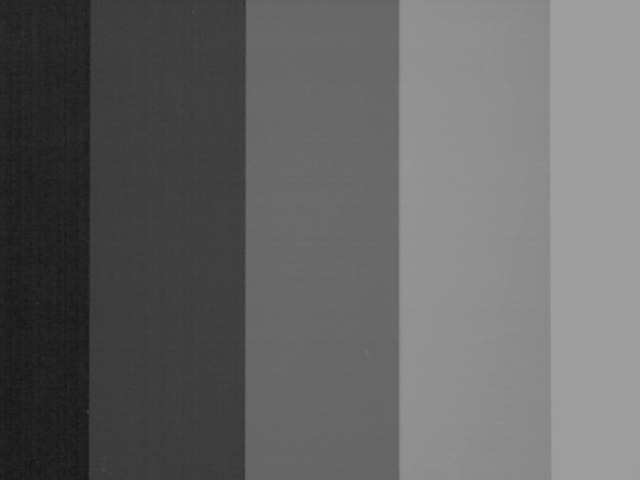
\includegraphics[width=\textwidth]{src/Grauwertkeil.png}
	\caption{Aufgenommener Grauwertkeil}
	\label{fig:GRAUWERTKEIL}
\end{figure}



\section{Auswertung}
\label{chap:VERSUCH_1_AUSWERTUNG}
In der Tabelle \ref{tab:Unterbilder} wird der Mittelwert und die Standardabweichung pro Unterbild abgebildet. In Listing \ref{lst:CodeV2} ist der zugehörige Code in der Methode 'versuch1()' zu finden.

\begin{table}[H]
\begin{tabular}{ccc}
\hline
\textbf{Stufe} &\textbf{ Mittelwert} & \textbf{Standardabweichung} \\
\hline
Unterbild 1 & 34.41 & 3.76 \\
\hline
Unterbild 2 & 62.49 & 1.77 \\
\hline
Unterbild 3 & 104.33 & 1.42 \\
\hline
Unterbild 4 & 142.01 & 2.66 \\
\hline
Unterbild 5 & 157.00 & 0.07 \\
\hline
\end{tabular} 
\caption{Unterbilder mit Mittelwert und Standardabweichung}
\label{tab:Unterbilder}
\end{table}

\section{Interpretation}
\label{chap:VERSUCH_1_INTERPRETATION}
Bezüglich des Mittelwertes aus Tabelle \ref{tab:Unterbilder} ist zu sagen, dass für Unterbild1 welches das dunkelste Bild ist der niedrigste Helligkeitswert angegeben ist. Für das Unterbild5 ist der höchste Wert zu erkennen. Bei einer möglichen Bandbreite von 0-255 Helligkeitsstufen ist die Aufnahme als kontrastarm zu interpretieren.
Bezüglich der Standardabweichung ist besonders das dunkle Unterbild1 mit einem hohen Abweichungsfaktor von fast 4 Helligkeitspunkten zu erkennen.
Diese höhere Abweichung könnte aufgrund von kratzen aber auch vom Sensorrauschen selbst sein. In der Abbildung \ref{fig:GRAUWERTKEIL} sind hellere Linien im Bild zu erkennen, die zu einer stärkeren Streuung des Helligkeitswertes beitragen.

%
% CHAPTER Versuch 2
%
\chapter{Versuch 2 - Aufnahme eines Dunkelbildes}
\label{chap:VERSUCH_2}
Nachfolgend wird ein Dunkelbild erzeugt, zur Eliminierung von Störgrößen in der Aufnahme, die z.B. durch Dunkelstrom verursacht werden.

\section{Fragestellung, Messprinzip, Aufbau, Messmittel}
\label{chap:VERSUCH_2_FRAGESTELLUNG}
Wie sieht ein passendes Dunkelbild zu dem Versuchsaufbau aus Versuch \ref{chap:VERSUCH_1} aus? Dabei wird thermisches Rauschen durch mehrere Messungen (10 Stück) und deren Mittlung eliminiert.\\
Messprinzip und Messmittel sind gleich zu Versuch \ref{chap:VERSUCH_1}.
Zu beachten ist bezüglich Aufbau, dass von den \textbf{gleichen} Belichtungsparametern und Entfernung der Kamera auszugehen ist.

\section{Messwerte}
\label{chap:VERSUCH_2_MESSWERTE}
Es wurden 10 Dunkelbilder aufgenommen und mit dem Mittelwert zu dem Bild in Abbildung \ref{fig:DunkelBildMittel} zusammengefügt.

\begin{figure}[H]
	\centering\small
	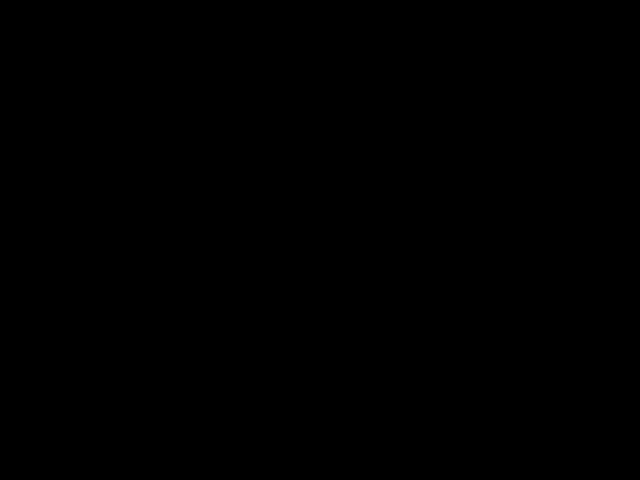
\includegraphics[width=\textwidth]{src/DunkelbildContrastMax.png}
	\caption{gemitteltes und kontrastmaximiertes Dunkelbild}
	\label{fig:DunkelBildMittel}
\end{figure}

\section{Auswertung}
\label{chap:VERSUCH_2_AUSWERTUNG}
Es wird der Mittelwert aus 10 Dunkelbildern pro Bildpunkt ermittelt und so ein Bild von Mittelwerten erstellt.
In Listing \ref{lst:CodeV2} ist der zugehörige Code in der Methode 'versuch2()' zu finden.

\section{Interpretation}
\label{chap:VERSUCH_2_INTERPRETATION}
Aufgrund der Bauart der Webkamera, dass besonders geringe Helligkeitswerte automatisch auf Null gesetzt werden, konnte die Ermittlung des Dunkelbildes nicht erfasst werden. Somit kommt es zu keiner Korrektur des Graukeils in den folgenden Versuchen durch das Dunkelbild. Es wird aber dennoch, aus theoretischen Sicht, mit dem Dunkelbild weitergearbeitet.\\
Desweiteren sind auch keine hot- oder stuckpixels aus den Werten zu erkennen.

%
% CHAPTER Versuch 3
%
\chapter{Versuch 3}
\label{chap:VERSUCH_3}

\section{Fragestellung, Messprinzip, Aufbau, Messmittel}
\label{chap:VERSUCH_3_FRAGESTELLUNG}

\section{Messwerte}
\label{chap:VERSUCH_3_MESSWERTE}

\section{Auswertung}
\label{chap:VERSUCH_3_AUSWERTUNG}

\section{Interpretation}
\label{chap:VERSUCH_3_INTERPRETATION}

%
% CHAPTER Versuch 4
%
\chapter{Versuch 4}
\label{chap:VERSUCH_4}

\section{Fragestellung, Messprinzip, Aufbau, Messmittel}
\label{chap:VERSUCH_4_FRAGESTELLUNG}

\section{Messwerte}
\label{chap:VERSUCH_4_MESSWERTE}

\section{Auswertung}
\label{chap:VERSUCH_4_AUSWERTUNG}

\section{Interpretation}
\label{chap:VERSUCH_4_INTERPRETATION}
%
% CHAPTER Anhang
%
\renewcommand\thesection{A.\arabic{section}}
\renewcommand\thesubsection{\thesection.\arabic{subsection}}

\chapter*{Anhang}
\label{chap:APPENDIX}
\addcontentsline{toc}{chapter}{Anhang}
%\setcounter{chapter}{0}
\addtocounter{chapter}{1}
\setcounter{section}{0}

\section{Quellcode}
\label{chap:APPENDIX_SOURCECODE}

\subsection{Quellcode Versuch 1}
\label{chap:APPENDIX_SOURCECODE_V1}
\begin{lstlisting}[style=PYTHON, frame=single, caption=QuellCodeV1 bis V4, captionpos=b, label=lst:CodeV2]
# -*- coding: utf-8 -*-
"""
Created on Mon Nov  9 15:07:39 2015
@author: Julian Altmeyer, Marcel Kieser
"""

import numpy as np
import cv2

def getSubImages(pic):
    image1 = pic[:,0:70]
    image2 = pic[:,90:230]
    image3 = pic[:,250:390]
    image4 = pic[:,410:550]
    image5 = pic[:,570:640]
    return image1, image2, image3, image4, image5


def getMeanStd(img):
    return np.mean(img), np.std(img)


def getTableLatex(table):
    strTab = ""
    for i in range(len(table)):
        strTab += "Unterbild " + str(i+1) + \
                  " & {0:.2f} & {1:.2f} \\\\\n\\hline\n".format(table[i][0],  table[i][1])

    print(strTab)

def maxContrast(img):
    maxValue = np.max(img)
    minValue = np.min(img)
    newImage = np.copy(img)
    
    for y in range(newImage.shape[0]):
        for x in range(newImage.shape[1]):
            if (maxValue - minValue) != 0:
                newImage[y][x] = (img[y][x] - minValue) * (255.0 / (maxValue - minValue))
            else:
                newImage[y][x] = 0
    return newImage


def versuch1():
    grayImg = cv2.imread("Grauwertkeil.png")    
    grayImg = cv2.cvtColor(grayImg, cv2.COLOR_BGR2GRAY)
    sliceAndTableImg(grayImg)

def sliceAndTableImg(image):    
    img1, img2, img3, img4, img5 = getSubImages(image)
    
    table = []
    table.append(getMeanStd(img1))
    table.append(getMeanStd(img2))
    table.append(getMeanStd(img3))
    table.append(getMeanStd(img4))
    table.append(getMeanStd(img5))
    
    getTableLatex(table)


def versuch2():
    dunkelbild = maxContrast(getDunkelbild())
    cv2.imwrite("DunkelbildContrastMax.png", dunkelbild)

def versuch3():
    weissbild = maxContrast(removeOffset(getWeissbild()))
    cv2.imwrite("WeissbildContrastMax.png", weissbild)
        

def versuch4():
    grayImg = cv2.imread("Grauwertkeil.png")
    grayImg = cv2.cvtColor(grayImg, cv2.COLOR_BGR2GRAY)
    dunkelbild = getDunkelbild()
    weissbild = getWeissbild()
    correctImg = correctImage(grayImg, weissbild, dunkelbild)
    cv2.imwrite("KorrigierterGrauwertkeil.png", correctImg)
    sliceAndTableImg(correctImg)

def correctImage(img, weisb, dunkelb):
    a = img - dunkelb
    a = a / normiereWeissbild(weisb)
    return a    
    
def normiereWeissbild(weissbild):
    w = np.double(weissbild)
    w = np.divide(w, np.mean(w))
    return w

def getWeissbild():
    weissbilder = []
    #erzeuge meanImage    
    for i in range(10):
        weissbilder.append(cv2.imread("Weissbilder/Weissbild" + str(i) + ".png"))
    
    meanImage = np.zeros((480, 640), dtype=int)

    for weissbild in weissbilder:
        wbild = cv2.cvtColor(weissbild, cv2.COLOR_BGR2GRAY)
        meanImage += wbild
        
    meanImage = meanImage / len(weissbilder)
    return meanImage

def getDunkelbild():
    dunkelbilder = []
    #erzeuge meanImage    
    for i in range(10):
        dunkelbilder.append(cv2.imread("Dunkelbilder/Dunkelbild" + str(i) + ".png"))

    meanImage = np.zeros((480, 640), dtype=int)

    for dunkelbild in dunkelbilder:
        dbild = cv2.cvtColor(dunkelbild, cv2.COLOR_BGR2GRAY)
        meanImage += dbild     
    
    meanImage = meanImage / len(dunkelbilder)
    return meanImage
    
def removeOffset(eingabebild):
    return eingabebild - getDunkelbild()

def main():
    versuch1()
    versuch2()
    versuch3()
    versuch4() 

if __name__ == "__main__":
    main()

    
\end{lstlisting}
\subsection{Quellcode Versuch 2}
\label{chap:APPENDIX_SOURCECODE_V2}

\subsection{Quellcode Versuch 3}
\label{chap:APPENDIX_SOURCECODE_V3}

\subsection{Quellcode Versuch 4}
\label{chap:APPENDIX_SOURCECODE_V4}


\section{Messergebnisse}
\label{chap:APPENDIX_MEASUREMENT_SOURCE}

%
% Literaturverzeichnis
%
%
% Literaturverzeichnis
%
\phantomsection
\addcontentsline{toc}{chapter}{Literaturverzeichnis}
\bibliography{../references}
\newpage

\end{document}
%------------------------------------
% ╔═╗╔╗╔╔╦╗  ╔╦╗╔═╗╔═╗╦ ╦╔╦╗╔═╗╔╗╔╔╦╗
% ║╣ ║║║ ║║   ║║║ ║║  ║ ║║║║║╣ ║║║ ║ 
% ╚═╝╝╚╝═╩╝  ═╩╝╚═╝╚═╝╚═╝╩ ╩╚═╝╝╚╝ ╩ 
%------------------------------------